\section{}

Wir schreiben die Funktion \texttt{poisson\_solver} aus Abschnitt~4.8 nach Matlab (bzw.\ Octave) um:

\lstinputlisting[style=matlabcode, firstline = 1, lastline = 46]{chapter_08/exercise_08_42.m}

Wir testen die Funktion \texttt{poisson\_solver} zunächst an den in (1) gegebenen Funktionen $f(x,y) = 1.25 \cdot e^{x + y/2}$, $g = e^{x + y/2}$ mithilfe des folgenden Codes:

\lstinputlisting[style=matlabcode, firstline = 52, lastline = 55]{chapter_08/exercise_08_42.m}

Wir erhalten hierdurch den folgenden Graphen:

\begin{center}
  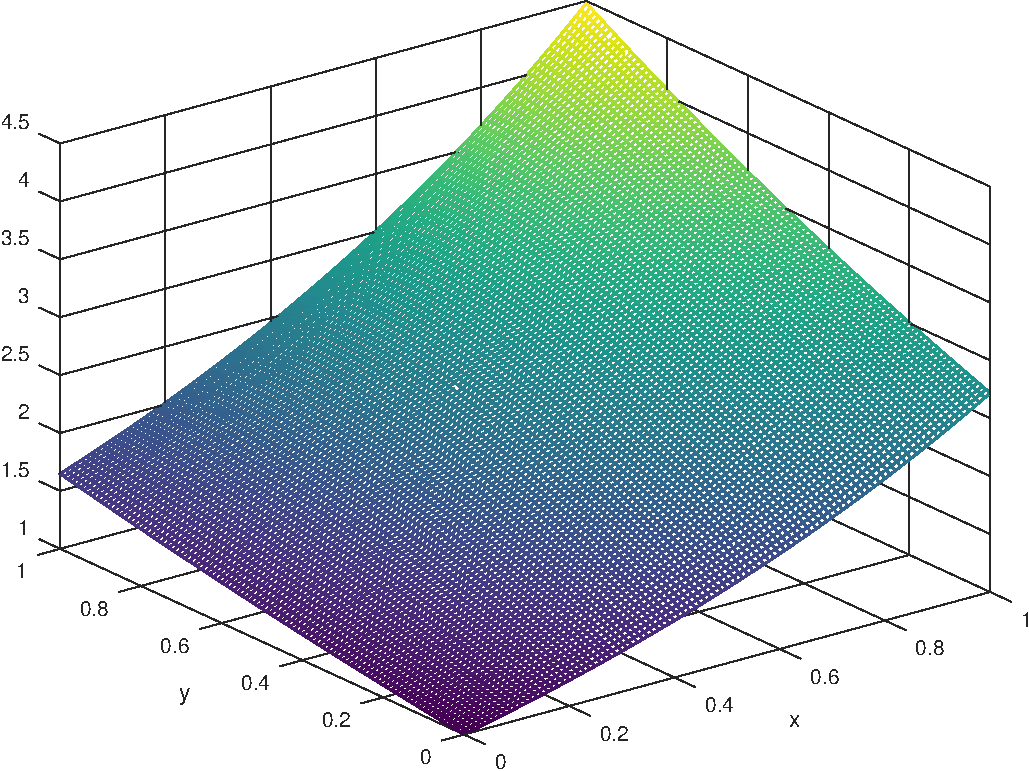
\includegraphics[width = \textwidth]{chapter_08/exercise_08_42_figure_1.pdf}
\end{center}

(Die auffällige weiße Lücke in der Mitte des Graphen entsteht beim Expotieren der Grafik aus Octave, und ist im Graphen selbst nicht vorhanden.)

Wir testen die Funktion \texttt{poisson\_solver} auch noch an in (2) gegebenen Funktionen.
Hierfür nutzen wir den folgenden Code:

\lstinputlisting[style=matlabcode, firstline = 61, lastline = 73]{chapter_08/exercise_08_42.m}

Wir erhalten hierdurch den folgenden Graphen:

\begin{center}
  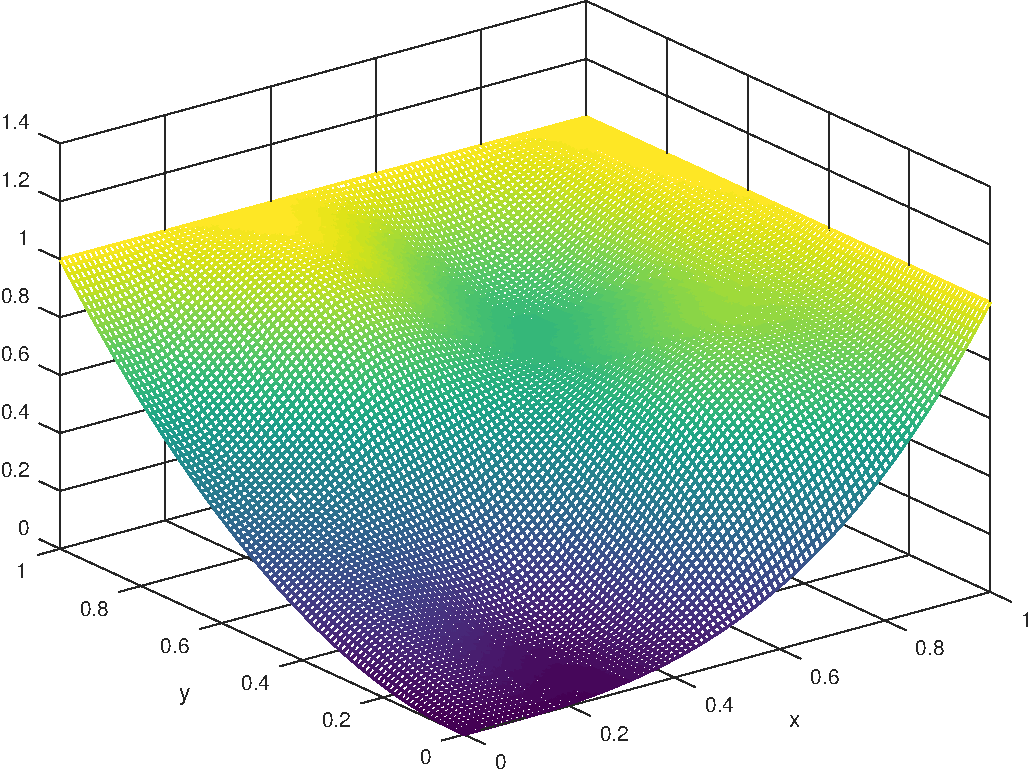
\includegraphics[width = \textwidth]{chapter_08/exercise_08_42_figure_2.pdf}
\end{center}
